\documentclass{article}
\usepackage{arxiv}

\usepackage[utf8]{inputenc}
\usepackage[english, russian]{babel}
\usepackage[T1]{fontenc}
\usepackage{url}
\usepackage{booktabs}
\usepackage{amsfonts}
\usepackage{bbm}
\usepackage{nicefrac}
\usepackage{microtype}
\usepackage{lipsum}
\usepackage{graphicx}
\usepackage{natbib}
\usepackage{doi}

\newcommand{\cmmnt}[1]{}

\title{Бэггинг над MARS со случайными поворотами признаков}

\author{ Додонов В.О.\\%David S.~Hippocampus\thanks{Use footnote for providing further
		%information about author (webpage, alternative
		%address)---\emph{not} for acknowledging funding agencies.} \\
	МГУ им. М.В. Ломоносова\\
	%Cranberry-Lemon University\\
	%Pittsburgh, PA 15213 \\
	\texttt{s02200360@gse.cs.msu.ru} \\
	%% examples of more authors
	\And
        Китов В.В.\\
	%Elias D.~Striatum \\
	%Department of Electrical Engineering\\
	%Mount-Sheikh University\\
	%Santa Narimana, Levand \\
        МГУ им. М.В. Ломоносова\\
	\texttt{v.v.kitov@yandex.ru} \\
	%% \AND
	%% Coauthor \\
	%% Affiliation \\
	%% Address \\
	%% \texttt{email} \\
	%% \And
	%% Coauthor \\
	%% Affiliation \\
	%% Address \\
	%% \texttt{email} \\
	%% \And
	%% Coauthor \\
	%% Affiliation \\
	%% Address \\
	%% \texttt{email} \\
}
\date{}

%\renewcommand{\shorttitle}{\textit{arXiv} Template}

%%% Add PDF metadata to help others organize their library
%%% Once the PDF is generated, you can check the metadata with
%%% $ pdfinfo template.pdf
\hypersetup{
pdftitle={Бэггинг над MARS со случайными поворотами признаков},
pdfsubject={q-bio.NC, q-bio.QM},
pdfauthor={David S.~Hippocampus, Elias D.~Striatum},
pdfkeywords={First keyword, Second keyword, More},
}

\begin{document}
\maketitle


\begin{abstract}
Алгоритм multivariate adaptive regression splines (MARS) обеспечивает гибкий
метод статистического моделирования, который использует прямой и обратный проходы, где происходит подбор порогов и переменных, для определения комбинации
базовых функций, которые наилучшим образом приближают исходные данные.
В области оптимизации MARS успешно использовался для оценки неизвестных функций в стохастическом динамическом программировании, стохастическом программировании и в других направлениях. MARS потенциально может быть полезен во многих реальных задачах оптимизации, где необходимо оценить целевую функцию на основе наблюдаемых данных. Однако использование MARS в ансамбле позволяет добиться даже большего качества на данных. Использование случайных ортогональных преобразований в ансамбле помогает сделать алгоритм менее чувствительным к расположению признаков в пространстве. Таким образом, получается найти более оптимальное приближение целевой функции в задаче регрессии.
\end{abstract}


\keywords{MARS \and Сплайны \and Регрессия \and Бэггинг \and Ансамбли}

\section{Введение}
%\lipsum[2]
%\lipsum[3]
В качестве популярного метода непараметрической регрессии алгоритм 
многомерных адаптивных регрессионных сплайнов (MARS) был впервые представлен Джеромом Фридманом в 1991 г. \cite{friedman1991multivariate}. Благодаря своей гибкости и точности MARS использовался во многих исследованиях, где возникает классическая для машинного обучения задача регрессии, включая прогнозирование спроса на энергию, необходимую для транспортировки \cmmnt{(M.A. Sahraei, H. Duman, M.Y. Çodur et al, 2021)} \cite{sahraei2021prediction}, анализ реакций роста, связанных с макропитательными веществами \cmmnt{(M Akin et al, 2020)} \cite{akin2020analysis}, построение системы принятия решений по борьбе с загрязнением озоном \cmmnt{(Yang, Chen, Chang, Sattler, \& Wen, 2009)} \cite{yang2009decision}, оценку подверженности овражной эрозии \cmmnt{(Conoscenti, Agnesi, Cama, Caraballo-Arias, \& Rotigliano, 2018)} \cite{conoscenti2018assessment}, оценку тепловой нагрузки в зданиях \cmmnt{(Roy, Roy, \& Balas, 2018)} \cite{roy2018estimating}, моделирование суточной концентрации растворенного кислорода \cmmnt{(Heddam \& Kisi, 2018)} \cite{heddam2018modelling} и др.
Также MARS используется и в медицинских целях, например, для выявления влияния пола на факторы, оказывающих воздействие на нарушения опорно-двигательного аппарата плеч, шеи и верхних конечностей
\cmmnt{(Serrano, Sanchez, Lasheras, Iglesias-Rodríguez, \& Valverde, 2020)} \cite{serrano2020identification}.

С момента появления классического алгоритма MARS~\cite{friedman1991multivariate} уже было произведено множество исследований, направленных на улучшение точности предсказания в задаче регрессии и ускорение обучения модели. Одними из первых стали модели с полиномиальными сплайнами \cite{stone1997polynomial}, в которой удаление базисной функции из алгоритма влекло за собой последующее удаление всех произведенных от нее элементов, и баесовская модификация MARS~\cite{denison1998bayesian}, где использовались марковские цепи и метод Монте-Карло.
Еще одним ответвлением стал CMARS~\cite{weber2012cmars}, использующий непрерывные методы оптимизации и регуляризации. 

Чтобы улучшить точность предсказаний алгоритма MARS и время обучения, были испробованы различные подходы. Например, ранее был предложен способ быстрой оптимизации узлов с использованием метода восхождения к вершине, где перебор порогов начинается с точки, на которой был достигнут максимум на предыдущем шаге \cmmnt{(Xinglong Ju, Victoria C.P. Chen, 2021)} \cite{ju2021fast}. Также в MARS можно использовать B-сплайны, что показало свою эффективность в решении задачи регрессии \cmmnt{(Sergey Bakin, Markus Hegland \& Michael R. Osborne, 2000)} \cite{bakin2000parallel}, либо другие улучшения, как Robust MARS \cmmnt{(Ozmen \& Weber, 2014)} \cite{ozmen2011rcmars}, который лучше справляется с менее надежными данными. Существую и другие подходы, расширяющие применение MARS, например, выпуклый вариант MARS, подходящий для решения специфических типов задач \cmmnt{(Martinez, Diana L., et al, 2015)}\cite{martinez2015convex}

В данной работе предлагается использовать бэггинг над MARS (Реализация PyEarth\footnote{\url{https://github.com/scikit-learn-contrib/py-earth}}), а так же использовать модификацию - случайный поворот признаков, на которых в последствии будет обучаться алгоритм. Предыдущие подходы не учитывали случай, предполагающий, что базисная функция может функционально зависеть от, например, некоторой линейной комбинации признаков. В таком случае целевая переменная не представима в виде базисных функций, которые предлагают строить другие подходы. Однако использование ансамбля моделей, где каждая модель использует свое собственное признаковое пространство, позволяет нивелировать данную проблему.

\section{Постановка задачи}
\label{sec:headings}

%\lipsum[4] See Section \ref{sec:headings}.
В задачах регрессии целевая переменная $y$ представляется в виде функции от $p$ переменных с некоторым шумом $\varepsilon$: $$y=f(x^1, x^2, ..., x^p) + \varepsilon,$$ где f неизвестная функция, и $\mathbbm{E}\varepsilon = 0$.

По рассматриваемому набору данных $D = \{x_i, y_i\}_{i=1}^{N}$, функция $f(x^1, x^2, ..., x^p)$ аппроксимируется некоторой функцией $g(x^1, x^2, ..., x^p)$. Качество аппроксимации оценивается с помощью среднего квадрата ошибки (MSE):
$$MSE(D) = \frac{1}{N}\sum_{k=1}^{N} (g(x_k) - y_k)^2$$
либо схожей величины $RMSE(D) = \sqrt{MSE(D)}$.
Считается, что модель с меньшим значением среднего квадрата ошибки лучше соответствует
данным.

В данной работе функция $g(x)$ строилась согласно алгоритму MARS (Multivariate Adaptive Regression Splines) \cite{friedman1991multivariate}, который аппроксимирует исходную функцию $f$ в виде:
$$h(x) = \sum_{m=0}^{M} a_m \cdot B_m(x),$$ где $B_m(x) = \prod_{k=1}^{K_m} b_{k,m}.$
$b_{k,m}$ - базисная функция от одной переменной, которая имеет вид либо $max\{+(x-t),~0\}$, либо $max\{-(x-t), 0\}.$

\section{Ансамбли и случайные повороты признаков}
В данной работе предлагается рассмотреть ансамблевые модели с использованием MARS с целью улучшения предсказательной способности классического алгоритма. В общем виде ансамблевые модели можно представить в виде:
$$M = R(a_1, a_2, ..., a_T),$$ где $a_t$ - базовые алгоритмы из некоторого рассматриваемого семейства $\mathcal{D}$. В данном случае предлагается рассмотреть:
\begin{equation} \label{eq:1}
    M(x) = \frac{1}{T}\sum_{t}^{T}a_t(x),
\end{equation}
где $M$ - полученная модель, $T$ - Количество базовых алгоритмов, $a_i$ - i-я базовая модель, построенная по алгоритму MARS.

Исходя из вида (\ref{eq:1}), в случае некоррелированности базовых моделей, разброс композиции (в силу разложения ошибки на смещение-разброс) должен убывать пропорционально $\frac{1}{T}$. Чтобы достичь меньшей корреляции между моделями, они обучаются на случайных подмножествах объектов (с повторениями) и случайных подмножествах признаков. 

Так как каждая базисная функция в MARS является функцией от одной переменной, получившаяся модель может по разному справляться с аппроксимацией функции от, например, линейной комбинации переменных. Чтобы разнообразить семейство алгоритмов и еще сильнее уменьшить корреляцию между моделями, предлагается рассматривать алгоритм MARS со случайными поворотами признаков. В общем случае матрицей поворота называется ортогональная матрица $Q$. Перед обучением алгоритма MARS можно производить преобразование признаков из набора данных $D$:
$\overline{x} = Qx$, где $Q$ - случайная ортогональная матрица, $QQ^T = I$, $x$ - $(x^1, ..., x^p)^T$ вектор в исходном пространстве признаков.

Матрица $Q$ генерируется из распределения Хаара. Матрицы из этого распределения можно получить следующим способом: если $A~\in~\mathbbm{R}^{n \times n}$, где каждый элемент сгенерирован независимо из стандартного нормального распределения, тогда матрица $Q$, участвующая в $QR$~-разложении $A$, - искомая матрица поворота.


\section{Эксперименты}
\subsection{Исходные данные и~условия эксперимента}
 
Для сравнения различных алгоритмов и подходов производились эксперименты на четырех различных наборах данных в задаче регрессии. Соответственно, во всех задачах в качестве метрики использовался RMSE.
Все рассматриваемые наборы данных представляют собой реальные выборки, в которых необходимо предсказывать вещественное число (Boston Housing (BH), California Housing (CH), Real estate price prediction (RE), Diabetes Dataset (DD)).

Во всех экспериментах исходный набор данных разбивался на 3 выборки:
обучающую, валидационную и тестовую. Соотношение между этими частями составляет 8:1:1 соответственно.

Размерность пространства признаков варьировалась от 6 до 10 в зависимости от задачи. В задачах применялась стандартизация наборов данных по обучающей выборке. 

Лучшие параметры модели подбирались по валидационной выборке, которые затем использовались для сравнения результатов на тесте.
Параметры бэггинга включают в себя следующие величины:
\begin{itemize}
    \item Количество базовых алгоритмов. Оптимальное значение зависит от задачи. Сотни базовых алгоритмов оказывалось достаточно.
    \item Доля признаков, которая выбиралась для обучения модели. В экспериментах наилучшее значение лежало в промежутке $[0.5, 1]$.
    \item Максимальное количество слагаемых в MARS. Использовались значения в диапазоне $[20, 40]$
    \item Использование случайных поворотов.
\end{itemize}

Для корректного анализа предсказательной способности моделей бэггинг над алгоритмами MARS сравнивался еще и с другими классическими моделями машинного обучения: случайный лес (RandomForest), градиентный бустинг (GradientBoosting), Ridge-регрессия. Аналогичным образом по валидационной выборке подбирались параметры максимальной глубины для случайного леса ($depth~\in~\{2,~4,~6,~8,~10\}$), шага обучения
($lr~\in~\{0.1,~0.3,~0.5\}$) и доли используемых объектов в обучении
($subsample~\in~\{0.7,~0.8,~0.9,~1\}$) для градиентного бустинга, коэффициента регуляризации ($C~\in~\{10^k:k=-3,...,4\}$) для Ridge-регрессии. 

\subsection{Результаты эксперимента}

\begin{figure}[H] %Разместить таблицу здесь
%\vskip-1cm \hskip-1.3cm
\begin{center}
    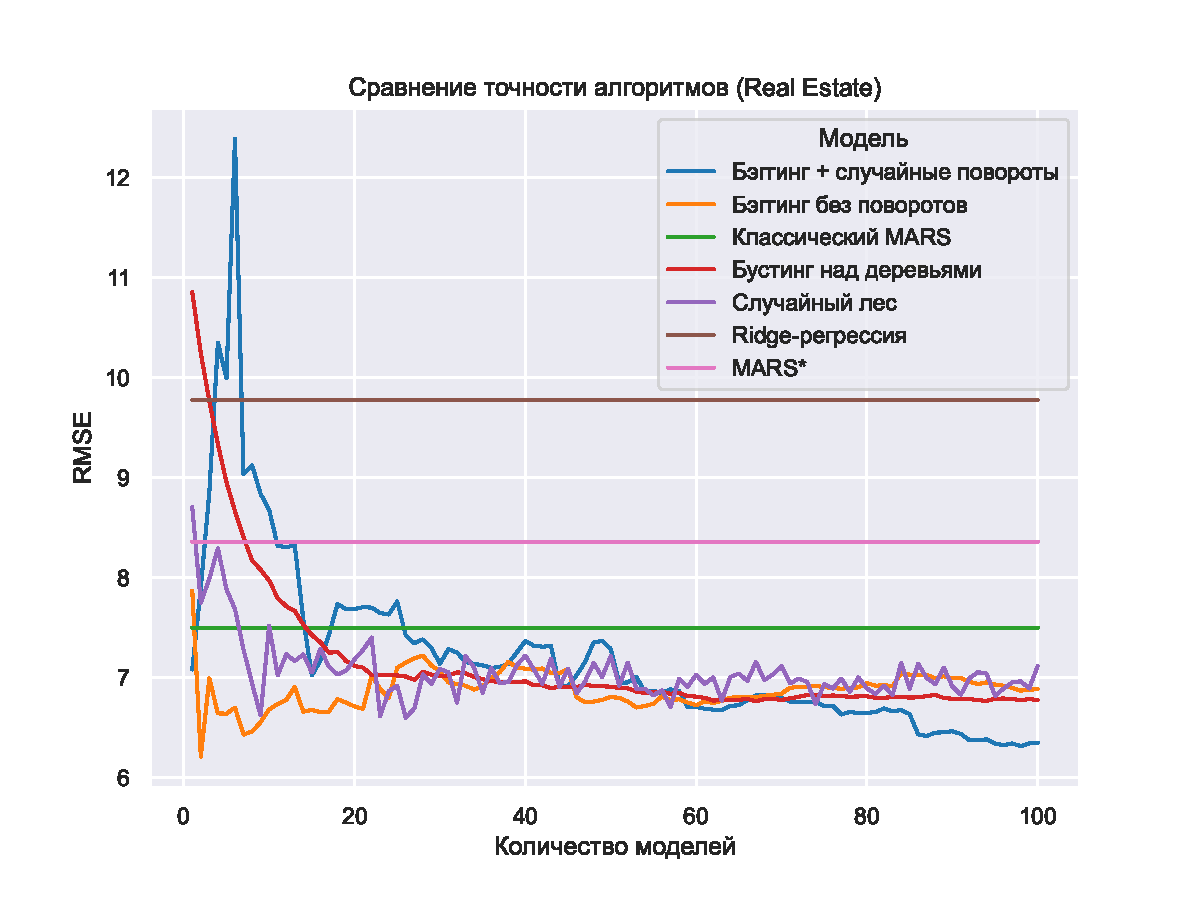
\includegraphics[scale=0.55]{figures/re_valmodels_2.pdf}
    \caption{Сравнение ансамблевого подходов с/без случайного поворота признаков со стандартным алгоритмом MARS и другими классическими алгоритмами машинного обучения (Набор данных - RE). Использовалось все признаковое пространство.}\label{fig::1}
\end{center}
\end{figure}
В результате эксперимента классический алгоритм оказался хуже ансамблевого подхода, который показал результат на валидационной (Рис. \ref{fig::1}) и тестовой выборках лучше (Табл. \ref{tab:1}).
Причем использование случайных поворотов позволило добиться меньшего значения RMSE на валидационной выборке, чем у градиентного бустинга. Также выяснилось, что с ростом числа базовых алгоритмов, использование случайных поворотов пространства признаков помогло улучшить предсказательную способность.

Рис. \ref{fig::2} иллюстрирует зависимость качества модель от используемых признаков. Использование части пространства признаков позволило уменьшить корреляцию между алгоритмами.

\begin{figure}[H] %Разместить таблицу здесь
%\vskip-1cm \hskip-1.3cm
\begin{center}
    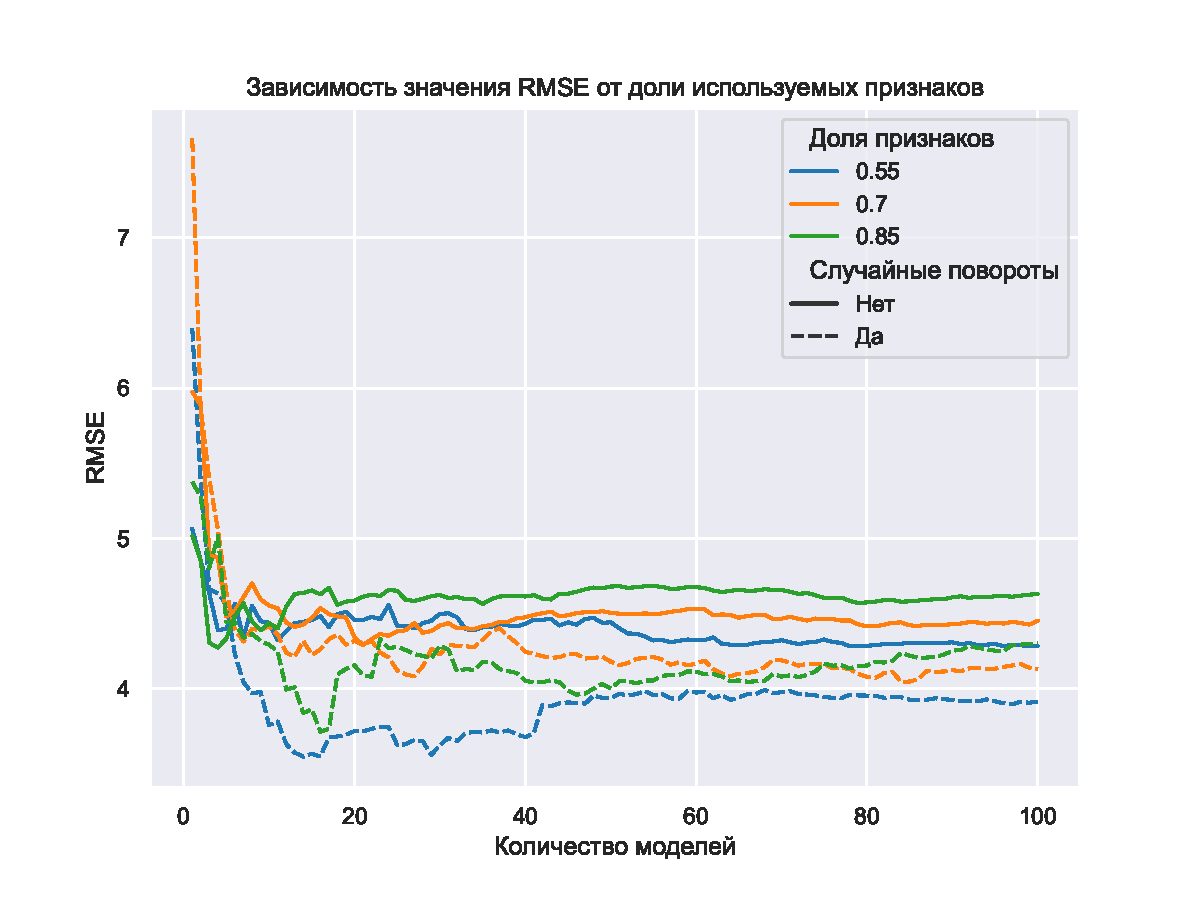
\includegraphics[scale=0.55]{figures/be_subsample.pdf}
    \caption{Влияние выбора доли используемых признаков в каждом базовом алгоритме ансамбля (Набор данных - BH). Классический алгоритм MARS достиг $RMSE = 4.402$}\label{fig::2}
\end{center}
\end{figure}

Результаты моделей, с наилучшими параметрами (с точки зрения качества на валидационной выборке) приведены в следующей Таблице (\ref{tab:1})
(MARS* соответствует модель, которая использовалась в качестве базового алгоритма в бэггинге):

\begin{table}[h!]
\begin{center}
\begin{tabular}{|c|c|c|c|c|}
\hline
Модель\textbackslashНабор данных & BH & CH & RE & DD\\
    \hline
    Классический MARS  & 3.09 &  0.66 &  5.27 &  53.5\\
    \hline
    MARS* & 3.32 &  0.67 &  6.08 &  57.2\\
    \hline
    Бэггинг без случайных поворотов  & \textbf{2.43} & 0.63 &  4.92 &  53.1\\
    \hline
    Бэггинг + 
    случайные повороты & 2.47 & 0.62 &  \textbf{4.48} &  \textbf{52.2}\\
    \hline
    Ridge-регрессия  & 5.41 &  0.75 &  6.81 &  58.3\\
    \hline
    Случайный лес  & 2.77 & 0.63 & 5.06 &  54.1\\
    \hline
    Бустинг над 
    деревьями & 2.51 &  \textbf{0.61} &  4.85 &  54.3\\
    \hline
\end{tabular}
\caption{\label{tab:1} Значение RMSE на тестовой выборке для каждой модели. Жирным выделен лучший результат.}
\end{center}
\end{table}


\subsection{Обсуждение и~выводы}

Таким образом, использование бэггинга над MARS на трех из четырех наборов данных позволило достичь лучшего результата на тестовой выборке. Однако стоит заметить, что в большинстве случаев именно подход со случайными поворотами признакового пространства помог добиться меньшего значения $RMSE$. То есть случайные повороты действительно смогли расширить семейство рассматриваемых базовых алгоритмов, уменьшив корреляцию между моделями.

Однако сложность построения ансамблевой модели составляет $\mathcal{O}(n)$, а если используется еще и матрица поворота, то появляются дополнительные затраты памяти порядка $\mathcal{O}(nd^2)$, где $n$ - количество базовых алгоритмов в ансамбле, $d$ - размерность пространства признаков. Бороться с этой проблемой можно, например, используя лишь некоторое подмножество матриц поворота

\section{Examples of citations, figures, tables, references}
\label{sec:others}

\subsection{Citations}
Citations use \verb+natbib+. The documentation may be found at
\begin{center}
	\url{http://mirrors.ctan.org/macros/latex/contrib/natbib/natnotes.pdf}
\end{center}

Here is an example usage of the two main commands (\verb+citet+ and \verb+citep+): Some people thought a thing \citep{kour2014real, hadash2018estimate} but other people thought something else \citep{kour2014fast}. Many people have speculated that if we knew exactly why \citet{kour2014fast} thought this\dots

\subsection{Figures}
\lipsum[10]
See Figure \ref{fig:fig1}. Here is how you add footnotes. \footnote{Sample of the first footnote.}
\lipsum[11]

\begin{figure}
	\centering
	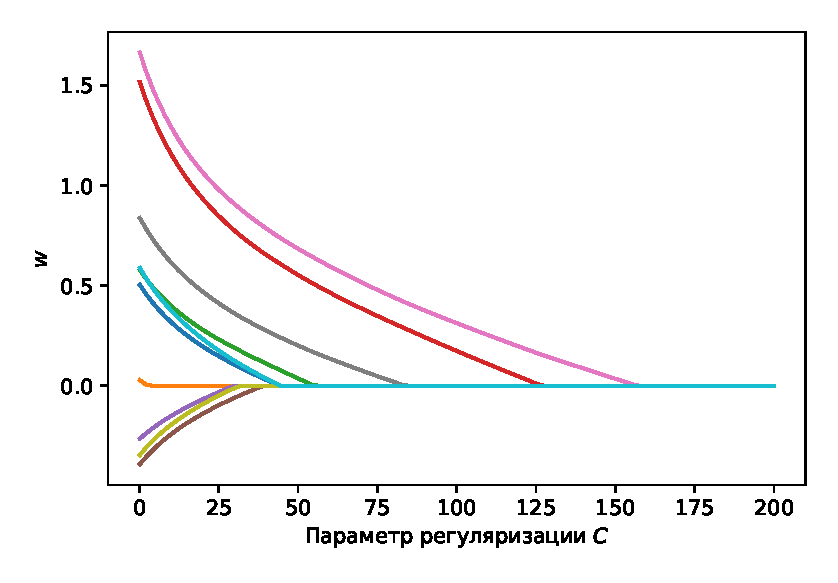
\includegraphics[width=0.5\textwidth]{../figures/log_reg_cs_exp.eps}
	\caption{Sample figure caption.}
	\label{fig:fig1}
\end{figure}

\subsection{Tables}
See awesome Table~\ref{tab:table}.

The documentation for \verb+booktabs+ (`Publication quality tables in LaTeX') is available from:
\begin{center}
	\url{https://www.ctan.org/pkg/booktabs}
\end{center}


\begin{table}
	\caption{Sample table title}
	\centering
	\begin{tabular}{lll}
		\toprule
		\multicolumn{2}{c}{Part}                   \\
		\cmidrule(r){1-2}
		Name     & Description     & Size ($\mu$m) \\
		\midrule
		Dendrite & Input terminal  & $\sim$100     \\
		Axon     & Output terminal & $\sim$10      \\
		Soma     & Cell body       & up to $10^6$  \\
		\bottomrule
	\end{tabular}
	\label{tab:table}
\end{table}

\subsection{Lists}
\begin{itemize}
	\item Lorem ipsum dolor sit amet
	\item consectetur adipiscing elit.
	\item Aliquam dignissim blandit est, in dictum tortor gravida eget. In ac rutrum magna.
\end{itemize}


\bibliographystyle{plain}
\bibliography{references}

\end{document}
